\documentclass[mini frame in current subsection]{beamer}
%\documentclass[10pt]{beamer}
\usepackage{url}
\usepackage{subfigure}
\usepackage{amssymb}
\usepackage{amsmath}
\usepackage{amsthm}
%\usepackage[dvips]{graphics}
%\usepackage{epsfig}
\usepackage{graphicx}
%\usepackage{graphics}
\usepackage[absolute,overlay]{textpos}
\usepackage{xcolor}
\usepackage{colortbl}
\usepackage{hhline}
\usepackage{multicol}
\newcommand{\lcdm}{$\Lambda$CDM }

%\input{../Paper/00a-Preamble/myFigures}
%\input{../Paper/00a-Preamble/myTables}
\usepackage[justification=centering]{caption}

\usepackage{amsthm}
\newtheorem{thm}{Theorem}

\usepackage{color}
\usepackage[absolute,overlay]{textpos}
\newenvironment{reference}[2]{%
  \begin{textblock*}{\textwidth}(#1,#2)
      \footnotesize\it\bgroup\color{white!50!blue}}{\egroup\end{textblock*}}


% You should run 'pdflatex' TWICE, because of TOC issues.

% Rename this file.  A common temptation for first-time slide makers is to name it something like ``my_talk.tex'' or ``john_doe_talk.tex'' or even ``discrete_math_seminar_talk.tex''.  You really won't like any of these titles the second time you give a talk.  Try naming your tex file something more descriptive, like ``riemann_hypothesis_short_proof_talk.tex''.  Even better (in case you recycle 99% of a talk, but still want to change a little, and retain copies of each), how about ``riemann_hypothesis_short_proof_MIT-Colloquium.2000-01-01.tex''?

\mode<presentation>
{
%\usetheme{progressbar}
  
  % A tip: pick a theme you like first, and THEN modify the color theme, and then add math content.
  % Warsaw is the theme selected by default in Beamer's installation sample files.

  %%%%%%%%%%%%%%%%%%%%%%%%%%%% THEME
%  \usetheme{Antibes}%Good but not better than JuanLesPins
%  \usetheme{Berlin}%Best so far
%  \usetheme{Copenhagen}%same as Berlin?
%  \usetheme{Darmstadt}%same as Berlin?
%  \usetheme{default}%No
%  \usetheme{Dresden}%Okay
%  \usetheme{Frankfurt}%Good, similar to Berlin
%  \usetheme{Goettingen}%Good for sidebar
%  \usetheme{JuanLesPins}%Good, similar to Berlin
  \usetheme[hideothersubsections]{Marburg}%Best sidebar so far
%	\usetheme{Rochester}
%	\beamertemplatenavigationsymbolsempty

  %%%%%%%%%%%%%%%%%%%%%%%%%%%% COLOR THEME
  %\usecolortheme{albatross}
  %\usecolortheme{beetle}
  %\usecolortheme{crane}
  %\usecolortheme{default}
  %\usecolortheme{dolphin}
  %\usecolortheme{dove}
  %\usecolortheme{fly}
  %\usecolortheme{lily}
  %\usecolortheme{orchid}
  %\usecolortheme{rose}
  %\usecolortheme{seagull}
  %\usecolortheme{seahorse}
  \usecolortheme{sidebartab}
  %\usecolortheme{structure}
  %\usecolortheme{whale}

  %%%%%%%%%%%%%%%%%%%%%%%%%%%% OUTER THEME
  %\useoutertheme{default}
  %\useoutertheme{infolines}
  \useoutertheme{miniframes}
  %\useoutertheme{shadow}
%  \useoutertheme{sidebar}
  %\useoutertheme{smoothbars}
  %\useoutertheme{smoothtree}
  %\useoutertheme{split}
  %\useoutertheme{tree}

  %%%%%%%%%%%%%%%%%%%%%%%%%%%% INNER THEME
  %\useinnertheme{circles}
  %\useinnertheme{default}
  %\useinnertheme{inmargin}
  \useinnertheme{rectangles}
  %\useinnertheme{rounded}

  %%%%%%%%%%%%%%%%%%%%%%%%%%%%%%%%%%%

  \setbeamercovered{transparent} % or whatever (possibly just delete it)
  % To change behavior of \uncover from graying out to totally invisible, can change \setbeamercovered to invisible instead of transparent. apparently there are also 'dynamic' modes that make the amount of graying depend on how long it'll take until the thing is uncovered.

}


% Get rid of nav bar
\beamertemplatenavigationsymbolsempty

%%% Use short top
\usepackage[headheight=12pt,footheight=12pt]{beamerthemeboxes}
\addheadboxtemplate{\color{black}}{
\hskip0.3cm
\color{white}
%\insertshortauthor \ \ \ \ 
%\includegraphics[scale=.4,clip]{Images/AFlogo.pdf}
\insertframenumber \ \ \ \ \ \ \ 
\insertsection \ \ \ \ \ \ \ \ \ \ \ \ \ \  \insertsubsection \ \ \ \ \ \ \ \ \ \ \ \ \ \  \insertsubsubsection
%\insertsectionnavigationhorizontal{\paperwidth}{}{hskip0pt plus1filll}
\hskip0.3cm
}
%\setbeamertemplate{headline}
%{
%	\begin{beamercolorbox}{section in head/foot}
%		\vskip2pt\insertsubsectionnavigationhorizontal{\paperwidth}{}{}\vskip2pt
%	\end{beamercolorbox}
%}

%\addheadboxtemplate{\color{black}}{
%\color{white}
%\ \ \ \ 
%\insertsection
%}
%\addheadboxtemplate{\color{black}}{
%\color{white}
%\ \ \ \ 
%\insertsubsection
%}

% Insert frame number at bottom of the page.
%\usefoottemplate{\hfil\tiny{\color{black!90}\insertframenumber}} 

\newcommand{\myToc}[1]
{
	\AtBeginSection[]
	{
		\begin{frame}
		\frametitle{#1}
		%\tableofcontents[currentsection,currentsubsection,subsectionstyle=show/show/hide]
		\tableofcontents[
		sectionstyle=show/shaded,
		subsectionstyle=show/show/hide,
		subsubsectionstyle=show/show/show/shaded
		]
		\end{frame}
	}
}

\myToc

\usepackage[english]{babel}
\usepackage[latin1]{inputenc}

\usepackage{times}
\usepackage[T1]{fontenc}

\title{MS-BANA and MS-IS Orientation}
\subtitle{Python Overview}

\author{Andrew Armstrong}

\institute{University of Cincinnati\\ Carl H. Lindner College of Business}

\date{2017 August 12}

%\subject{Course Introduction and Overview}

\def\defn#1{{\color{red} #1}}

\begin{document}

\begin{frame}
  \titlepage
\end{frame}

\section{Introduction}

	\subsection{Education}

		\begin{frame}
			\frametitle{Education}
				\begin{itemize}
					\item  Dual Bachelors in Computer Engineering and Mathematics
						\begin{itemize}
							\item Michigan Technological University			
						\end{itemize}
					\item  Masters in Computer Engineering
						\begin{itemize}
							\item  The Air Force Institute of Technology
							\item  Thesis work focusing on cryptanalysis
						\end{itemize}
					\item  Masters in Management of Technology
						\begin{itemize}
							\item  University of Texas at San Antonio
						\end{itemize}
					\item  PhD in Applied Mathematics
						\begin{itemize}
							\item  The Air Force Institute of Technology
							\item  Dissertation work focusing on the analysis of of astronomical data
						\end{itemize}
				\end{itemize}
		\end{frame}
		
	\subsection{Contact Information}
		\begin{frame}
			\frametitle{Contact Information}
				\begin{itemize}
					\vfill\item  School email:  
						\begin{itemize}
							\item  \href{mailto:armstam@ucmail.uc.edu}{armstam@ucmail.uc.edu}
						\end{itemize}
					\vfill\item  Personal email:  
						\begin{itemize}
							\item  \href{mailto:andrewarmstrong004@gmail.com}{andrewarmstrong004@gmail.com}
						\end{itemize}
				\end{itemize}\vspace{2.5em}
		\end{frame}
		
\section{Course Website}
	\subsection{Course Website}
	
		\begin{frame}
			\frametitle{Course Resources}
			\begin{itemize}
				\vfill\item  You can find all the material for this course at the following website.
				\vfill\item  \url{https://github.com/andrewarmstrong004/MS-BANA-Orientation}
			\end{itemize}
		\end{frame}
		
	
	\subsection{Course Description and Objectives}
		\begin{frame}
			\frametitle{Course Description}
			
				This course is designed to be an introduction to Python for applications in data analytics.  The material will emphasize the core concepts in Python, specifically data types, data structures, and functions and how they can be implemented and used to address data analytics problems.  Popular modules used in data analysis will also be covered at a high level.
				
		\end{frame}
		
		\begin{frame}
			\frametitle{Course Objectives}
			\begin{itemize}
				\item Course Objectives
					\begin{itemize}
						\vfill\item  Describe the differences between the main branches of Python
						\vfill\item  Know and be able to utilize the basic Python data types and structures
						\vfill\item  Write basic Python statements such as if/elif/else, for loops, and while loops
						\vfill\item  Be able to import and use standard Python modules for importing, exporting, and manipulating data
						\vfill\item  Write a basic Python module and be able to describe how modules work
						\vfill\item  Incorporate commonly used modules into a program to improve its utility
					\end{itemize}
			\end{itemize}
		\end{frame}
		
	\subsection{Course References}
		\begin{frame}
			\frametitle{Course References}

			\begin{itemize}
				\vfill\item Python Basics - \textbf{Main book for the course}
					\begin{itemize}
						\item  Lutz, Mark, {\textit{Learning Python}}, O'Reilly Media, 5th Edition, 2013.
					\end{itemize}
				\vfill\item Python Analytics
					\begin{itemize}
						\item McKinney, Wex, {\textit{Python for Data Analysis: Data Wrangling with Pandas, NumPy, and IPython}}, O'Reilly Media, 1st Edition, 2012.
						\item  Grus, Joel, {\textit{Data Science from Scratch:  First Principles with Python}}, O'Reilly Media, 1st Edition, 2015.
					\end{itemize}
				\end{itemize}
		\end{frame}
		
		\begin{frame}
			\frametitle{Course References Continued}
			\begin{itemize}
				\vfill\item More Advanced Python
					\begin{itemize}
						\item  Lutz, Mark, {\textit{Programming Python: Powerful Object-Oriented Programming}}, O'Reilly Media, 4th Edition, 2011.
						\item  Slatkin, Brett, {\textit{Effective Python: 59 Specific Ways to Write Better Python}}, Addison-Wesley Professional, 1st Edition, 2015.
					\end{itemize}
				\vfill\item  Transitioning from Python 2.7x to Python 3.x
					\begin{itemize}
						\item  Ramalho, Luciano, {\textit{Fluent Python: Clear, Concise, and Effective Programming}}, O'Reilly Media, 1st Edition, 2015.
					\end{itemize}
				\vfill\item  Theory
					\begin{itemize}
						\item  Hastie, Trevor et al., {\textit{The Elements of Statistical Learning: Data Mining, Inference, and Prediction}}, Springer, 2nd Edition, 2016.
				\end{itemize}
			\end{itemize}
		\end{frame}
		
	\subsection{Tentative Course Outline}
		\begin{frame}
			\frametitle{Tentative Course Outline - Day 01}
			\begin{itemize}
				\item  Basic introduction to Python
				\item  Where to write Python code
				\item  Creating your first program
				\item  Overview of boolean and numeric types
				\item  Introduction to function
				\item  Control flow
				\item  Sequences, Sets, and Mappings
				\item  Data I/O
				\item  Loops
				\item  Advanced functions
				\item  Plotting
				\item  Regression
				\item  Data science modules
				\item  Useful functions
			\end{itemize}
		\end{frame}

\section{Overview of Python}
	\subsection{Installing Anaconda}
	
		\begin{frame}
			\frametitle{Installing Anaconda}
			\begin{itemize}
				\vfill \item Download Anaconda from 
					\begin{itemize}
						\item \url{https://www.continuum.io/downloads}
					\end{itemize}
				\vfill \item  Make sure that you are downloading version 2.7x
					\begin{itemize}
						\item This should be the lower download button (should be blue)
					\end{itemize}
				\vfill \item  Anaconda bundles up Python and several commonly used modules into single file for easy download
					\begin{itemize}
						\item  List of packages included in Anaconda: \url{https://docs.continuum.io/anaconda/pkg-docs}
						\item  These packages bring a lot of functionality to Python that we can take advantage of, however, they are not all the possible Python packages that you could use
					\end{itemize}
				\vfill \item  Once you have it fully downloaded, just leave it, we will take care of it later
			\end{itemize}
		\end{frame}
		
	\subsection{Python History}
	
		\begin{frame}
			\frametitle{Python History}
			\begin{itemize}
				\vfill \item  Originally written by Guido van Rossum
					\begin{itemize}
						\item  Guido van Rossum worked at Centrum Wiskunde \& Informatica (CWI) in the Netherlands
						\item Development started over the Christmas break in 1989 as a "hobby" programming project to work on during his time off
					\end{itemize}
				\vfill \item  Python is the successor of the ABC language, which was also written by workers at CWI
				\vfill \item  Python is named after Monty Python's Flying Circus, not after the snake
			\end{itemize}
		\end{frame}
	
		\begin{frame}
			\frametitle{Python Development}
			\begin{itemize}
				\vfill \item  Python version 0.9.0, the first publicly available version, was released in February 1991 on alt.sources
					\begin{itemize}
						\item  Included classes and inheritance
						\item  Included core data data types \texttt{list}, \texttt{dict}, and \texttt{str}
					\end{itemize}
				\vfill \item  Version 1.0 was released in January of 1994
					\begin{itemize}
						\item Major additions included \texttt{lamda}, \texttt{map}, \texttt{filter}, and \texttt{reduce}
					\end{itemize}
				\vfill \item  Version 2.0 was released in October of 2000
					\begin{itemize}
						\item  Introduced list comprehensions, which is a fancy way of making lists
					\end{itemize}
			\end{itemize}
		\end{frame}
	
		\begin{frame}
			\frametitle{Python 2.7x vs Python 3.x}
			\begin{itemize}
				\vfill \item  Python 2.6 and 3.0 were released simultaneously in December of 2008
					\begin{itemize}
						\item  The split in versions was due to the fixing in some design flaws built into Python which didn't allow for complete backwards compatibility
						\item  Python 3 attempted to ``reduce feature duplication by removing old ways of doing things''
					\end{itemize}
				\vfill \item  Python 2.7 and 3.1 releases coincided in June of 2009
					\begin{itemize}
						\item  This is the last major release of Python 2.x
					\end{itemize}
				\vfill \item  In November of 2014 it was announced that support of Python 2.7 would last until 2020
			\end{itemize}
		\end{frame}
	
	\subsection{Python Methodology}
	
		\begin{frame}
			\frametitle{The Zen of Python}
			\begin{itemize}
				\vfill \item  The core philosopy of Python is summarized in The Zen of Python (PEP 20)
					\begin{itemize}
						\item  \url{https://www.python.org/dev/peps/pep-0020/}
						\item  PEP stands for Python Enhancement Proposals
					\end{itemize}
				\vfill \item Examples from The Zen of Python include:
					\begin{itemize}
						\item  Beautiful is better than ugly
						\item  Explicit is better than implicit
						\item  Simple is better than complex
						\item  Complex is better than complicated
						\item  Readability counts
					\end{itemize}
			\end{itemize}
		\end{frame}
	
		\begin{frame}
			\frametitle{Python Features}
			\begin{itemize}
				\vfill \item  Python is a multi-paradigm programming language
					\begin{itemize}
						\item  Object-oriented programming
						\item  Structured programming
						\item  Functional programming
						\item  and many others
					\end{itemize}
				\vfill \item  Python uses dynamic typing
					\begin{itemize}
						\item Meaning you don't have to tell Python what type of variable you are making and that the type of variable can change
					\end{itemize}
				\vfill \item  Python has built in garbage collection
					\begin{itemize}
						\item  This means Python cleans up its own memory
						\item  Done using reference counting and a cycle-detection garbage collector
					\end{itemize}
			\end{itemize}
		\end{frame}
	
		\begin{frame}
			\frametitle{Pythonic Way of Thinking}
			\begin{itemize}
				\vfill \item  Pythonic means code that doesn't just get the syntax right 
					\begin{itemize}
						\item Pythonic code follows the conventions of the Python community and uses the language in the way it is intended to be used.
					\end{itemize}
				\vfill \item  Python was made to be extended
				\vfill \item  This means that all desired components of the language don't need to be built into the languages core
				\vfill \item  Python was written to be easily read and fun to use
					\begin{itemize}
						\item  Many online examples use references to Monty Python for example
					\end{itemize}
			\end{itemize}
		\end{frame}
		
	
	\subsection{Python Applications}
	
		\begin{frame}
			\frametitle{Python Applications}
			\begin{itemize}
				\vfill \item  System programming
					\begin{itemize}
						\item  System administration tools
					\end{itemize}
				\vfill \item  Graphical User Interfaces (GUIs)
					\begin{itemize}
						\item  Making pretty user interfaces
					\end{itemize}
				\vfill \item  Internet scripting
					\begin{itemize}
						\item  Networking tasks
					\end{itemize}
				\vfill \item  Component integration
					\begin{itemize}
						\item  ``Gluing'' different pieces of code, even from different languages, together
					\end{itemize}
				\vfill \item  Numeric and scientific computing
					\begin{itemize}
						\item  Competing with even C++ and FORTRAN
					\end{itemize}
			\end{itemize}
		\end{frame}
	
		\begin{frame}
			\frametitle{Python Applications}
			\begin{itemize}
				\vfill \item  Rapid prototyping
					\begin{itemize}
						\item  Fast initial development with easy transition to other languages like C
					\end{itemize}
				\vfill \item  Database programming
					\begin{itemize}
						\item  Managing large databases
					\end{itemize}
				\vfill \item  Game design
					\begin{itemize}
						\item  Creating games, even complex and attractive games
					\end{itemize}
				\vfill \item  Data mining
					\begin{itemize}
						\item  Fast and easy data mining applications
					\end{itemize}
				\vfill \item  Robotics
					\begin{itemize}
						\item  Controlling robotic systems
					\end{itemize}
			\end{itemize}
		\end{frame}
		
	\subsection{Python in the Real World}
	
		\begin{frame}
			\frametitle{Python in the Real World}
			\begin{itemize}
				\vfill \item  Google
					\begin{itemize}
						\item  Extensively uses Python in its web search system
					\end{itemize}
				\vfill \item  YouTube
					\begin{itemize}
						\item  Largely written in Python
					\end{itemize}
				\vfill \item  Dropbox
					\begin{itemize}
						\item  Server and desktop client written primarily in Python
						\item  Guido van Rossum now works for Dropbox
					\end{itemize}
				\vfill \item  Raspberry Pi
					\begin{itemize}
						\item  Promotes python as its educational language
					\end{itemize}
				\vfill \item  EVE Online (a massively multiplayer online game)
					\begin{itemize}
						\item  Broadly uses python
					\end{itemize}
			\end{itemize}
		\end{frame}
	
		\begin{frame}
			\frametitle{Python in the Real World}
			\begin{itemize}
				\vfill \item  BitTorrent
					\begin{itemize}
						\item  First began as a Python program
					\end{itemize}
				\vfill \item  Industrial Light \& Magic
					\begin{itemize}
						\item  Uses Python in the production of movies
					\end{itemize}
				\vfill \item  NSA
					\begin{itemize}
						\item  Cryptographic and intelligence analysis
					\end{itemize}
				\vfill \item  One Laptop Per Child (OLPC)
					\begin{itemize}
						\item  Used to build the user interface
					\end{itemize}
				\vfill \item  JPMorgan Chase
					\begin{itemize}
						\item  Financial market forecasting
					\end{itemize}
			\end{itemize}
		\end{frame}
		
	\subsection{Documentation and Resources}
	
		\begin{frame}
			\frametitle{Documentation}
			\begin{itemize}
				\vfill \item  The core documentation for Python is located at: \url{https://docs.python.org/2.7/}
				\vfill \item  Reading this documentation can be relatively challenging, but is really worth the effort
				\vfill \item  If you don't want to dig through all the technical background of a function, and just want the answer, Google is your friend
				\vfill \item  Most Google searches will lead you to \url{https://stackoverflow.com}
					\begin{itemize}
						\item  For example:  \url{https://goo.gl/c9pYY6}
					\end{itemize}
			\end{itemize}
		\end{frame}
	
		\begin{frame}
			\frametitle{Getting Help in Python}
			\begin{itemize}
				\vfill \item  \texttt{help()}
					\begin{itemize}
						\item  Gives you help about a function or class
						\item  Typing in just help()
						\item  Typing in help(list)
					\end{itemize}
				\vfill \item  \texttt{dir}
					\begin{itemize}
						\item  Tells you the attributes of the function or class
						\item  Type dir(list)
					\end{itemize}
				\vfill \item  \texttt{dict}
					\begin{itemize}
						\item  The attribute dictionary of a function or class
						\item  Type list.\_\_dict\_\_
					\end{itemize}
				\vfill \item  Easiest way is to Google it or look up the documentation online
			\end{itemize}
		\end{frame}
		
	\subsection{Finalizing Anaconda Installation}
	
		\begin{frame}
			\frametitle{Finalizing Anaconda Install}
			\begin{itemize}
				\vfill \item  \url{https://www.continuum.io/downloads}
				\vfill \item  Adding it to your path
					\begin{itemize}
						\item Linux:  \texttt{export PATH="/Users/jsmith/anaconda2/bin:\$PATH"}
						\item Windows don't worry about it
					\end{itemize}
				\vfill \item  \texttt{conda create --name snowflakes}
			\end{itemize}
		\end{frame}
		
\section{Writing Python Code}

	\subsection{Class Folder Setup}
	
		\begin{frame}
			\frametitle{Class Folder Setup}
			
			\begin{itemize}
				\vfill\item  Create a folder in a location easily navigated to
					\begin{itemize}
						\item  We will use this folder over the course of the day
						\item  This folder should be in the same drive as your Anaconda installation
					\end{itemize}
				\vfill\item  Navigate to \url{https://github.com/andrewarmstrong004/MS-BANA-Orientation}
				\vfill\item  This site has all the material you will need for class today
				\vfill\item  Download at least the first couple lecture and practice files
					\begin{itemize}
						\item  These files should end with .ipynb
					\end{itemize}
			\end{itemize}
			
		\end{frame}
	\subsection{Using the Terminal}
	
		\begin{frame}
			\frametitle{Using the Terminal}
			\begin{itemize}
				\vfill \item  Open up your python terminal
					\begin{itemize}
						\item  Either type in conda
						\item  Or open up the terminal from your application launcher
					\end{itemize}
				\vfill \item  \texttt{$>>>$} means you are in a python environment
					\begin{itemize}
						\item  if you don't see that, something is wrong
					\end{itemize}
				\vfill \item  type the following into your terminal:
					\begin{itemize}
						\item  \texttt{$>>>$ print `Hello, World!'}
					\end{itemize}
				\vfill \item  Congratulations, your just wrote your first Python code
			\end{itemize}
		\end{frame}
		
	\subsection{Text Editor}
	
		\begin{frame}
			\frametitle{Using a Text Editor}
			\begin{itemize}
				\vfill \item  You can also just write Python code in a text editor and save it as a .py file
				\vfill \item  You can then just run this Python file by typing in \texttt{python python\_file.py} into your terminal
				\vfill \item  This is not recommended, it is very hard to problem solve this way
					\begin{itemize}
						\item  Especially getting rid of nuisance whitespace
					\end{itemize}
			\end{itemize}
		\end{frame}
		
	
		\begin{frame}
			\frametitle{Using a Text Editor}
			\begin{itemize}
				\vfill \item  Open up a new blank document in a basic text editor, like notepad on windows
				\vfill \item  type the following code into your new document:
					\begin{itemize}
						\item  \texttt{print `Hello, World!'}
						\item  \texttt{print 5+7}
					\end{itemize}
				\vfill \item  Save this new file as first\_python\_program.py on your desktop or in an easily to navigate to folder
				\vfill \item  Open up your Anaconda terminal and navigate to your new file

				\vfill \item  Once there, execute the following command:
					\begin{itemize}
						\item  python first\_python\_program.py
					\end{itemize}
				\vfill \item  You now have written your first Python program
			\end{itemize}		
				
		\end{frame}
		
	\subsection{Integrated Development Environments (IDEs}
	
		\begin{frame}
			\frametitle{Integrated Development Environments (IDEs}
			\begin{itemize}
				\vfill \item  IDEs are very common ways of programming in Python
				\vfill \item  Common IDEs include:
					\begin{itemize}
						\item  Spyder:  \url{https://pythonhosted.org/spyder/}
							\begin{itemize}
								\item  Should be installed with Anaconda
							\end{itemize}
						\item  Notepad++:  \url{https://notepad-plus-plus.org/download/v7.3.3.html}
						\item  Sublime Text:  \url{http://www.sublimetext.com/2}
						\item  PyCharm:  \url{https://www.jetbrains.com/pycharm/}
							\begin{itemize}
								\item  The one I use most often
								\item  I believe its free for students
							\end{itemize}
					\end{itemize}
				\vfill \item  Find one you like and try to learn all its bells and whistles
			\end{itemize}
		\end{frame}
		
	
		\begin{frame}
			\frametitle{Integrated Development Environments (IDEs}
			\begin{itemize}
				\vfill \item  Open up your favorite Python IDE
					\begin{itemize}
						\item  If you haven't used Python before, open up the Spyder program that comes with Anaconda
						\item  If using Windows, Spyder should be located in the Anaconda folder in your Start menu
					\end{itemize}
				\vfill \item  Type the example code into the appropriate area of your IDE
					\begin{itemize}
						\item  Take note of the difference in color and formatting when using an IDE when compared to notepad (or similar)
					\end{itemize}
				\vfill \item  Save the code as second\_python\_program.py in an easily accessible area
				\vfill \item  Run the code using your terminal or with the built in functions of your IDE
					\begin{itemize}
						\item  If you are using your terminal, type the following into it:
							\begin{itemize}
								\item  python second\_python\_program.py
							\end{itemize}
					\end{itemize}
			\end{itemize}
		\end{frame}
		
%	\subsection{Python Notebooks}
	
		\begin{frame}
			\frametitle{Python Notebooks}
			\begin{itemize}
				\vfill \item  In Windows you can just open jupyter notebooks from the Start menu
				\vfill \item  Using your terminal, navigate to your desired folder for class
				\vfill \item  type \texttt{jupyter notebook} in the terminal
			\end{itemize}
		\end{frame}
	
		\begin{frame}
			\frametitle{Python Notebooks}
			\begin{itemize}
				\vfill \item  Once you have Jupyter Notebooks open, use the file navigation system to navigate to the folder we setup earlier
					\begin{itemize}
						\item  The folder that you have been saving the .ipynb files to
					\end{itemize}
				\vfill\item  Open Lecture 00 - Third Python Program
				\vfill\item  Use the command shift+enter to execute the code selected and move on to the next section
				\vfill\item  Use the command ctrl+enter to execute the code selected, but stay on the same code block
				\vfill\item  Press h when not in edit mode to see all the command shortcuts
				\vfill\item  Execute the first three code blocks
				\vfill\item  Change the name in the forth code block to be your own name and execute the code
			\end{itemize}
		\end{frame}
	
		\begin{frame}
			\frametitle{Python Notebooks}
			\begin{itemize}
				\vfill \item  In Windows you can just open jupyter notebooks from the Start menu
				\vfill \item  Using your terminal, navigate to your desired folder for class
				\vfill \item  type \texttt{jupyter notebook} in the terminal
			\end{itemize}
		\end{frame}
	
		\begin{frame}
			\frametitle{Python Notebooks}
			\begin{itemize}
				\vfill \item  Python notebooks are good places to write code when you are building and testing new code
				\vfill\item  They are also very helpful when you need to share code or write up examples of code
				\vfill\item  We will be using jupyter notebooks for nearly all the code in this class, however, they may not be optimal for writing up code for actual implementation
				\vfill\item  For actual implementation, writing up code using an IDE is usually the prefered method
					\begin{itemize}
						\item  But even very strong python programmers use notebooks to build and test before implementation in a python file
					\end{itemize}
			\end{itemize}
		\end{frame}
		
	\subsection{White Space}
	
		\begin{frame}
			\frametitle{A Note on the Importance of Whitespace}
			\begin{itemize}
				\vfill \item  Python is one of the few languages where whitespace matters
				\vfill \item  This means that you can't just add random indentation to your code like you can in other languages
				\vfill \item  Python does this to both make the code easier to read and to get away from all the parenthesis and similar symbols scattered throughout most other languages
				\vfill\item  This becomes very important when dealing with control flow, functions, and loops
			\end{itemize}
		\end{frame}

\section{Code Examples and Practice}

	\subsection{Boolean and Numeric Types}
	
		\begin{frame}
			\frametitle{Lecture 01 - Boolean and Numeric Types}
			\begin{itemize}
				\vfill\item  In this section we are going to cover the most basic data types used in Python
				\vfill\item  Boolean Types
					\begin{itemize}
						\item  boolean
						\begin{itemize}
							\item  A boolean is either True of False
							\item  Can also be thought of as a $1$ or $0$
							\item  Examples:  True, False
						\end{itemize}
					\end{itemize}
				\vfill\item  Numeric Types
					\begin{itemize}
						\item  Integer
							\begin{itemize}
								\item  This is a whole number, or a natural number
								\item  Examples:  $0$, $1$, $-17$, $1287$
							\end{itemize}
						\item  Floating Point Number
							\begin{itemize}
								\item  This is a number with a trailing decimal point
								\item  Examples:  $0.0$, $1.0$, $.333333$, $3.1415926$
							\end{itemize}
						\item  Complex Number
							\begin{itemize}
								\item  Numbers with an imaginary component
								\item  Examples:  $1+1j$, $3j$, $2.7+.8j$
							\end{itemize}
					\end{itemize}
			\end{itemize}
		\end{frame}
		
		
	
		\begin{frame}
			\frametitle{Naming Variables}
			\begin{itemize}
				\vfill\item  We can store information in Python by naming variables and assigning them values
				\vfill\item  A basic example would be:  \texttt{a = 7}
				
				\vfill\item  In Python we do not need to type cast variables, meaning we don't need to tell Python what type of variable we are going to be needing (like an int of bool)
				
				\vfill\item  We can also reassign variables to be a completely different type by just reassigning it
					\begin{itemize}
						\item  \texttt{a = 2.4}
					\end{itemize}
			\end{itemize}
		\end{frame}
		
		
	
		\begin{frame}
			\frametitle{Mutability}
			\begin{itemize}
				\vfill\item  Once a variable is assigned it creates a point in memory where it stores the data
				\vfill\item  It then creates a pointer with the given name which points to that location
				\vfill\item  To change what a given variable is pointing at, we then have two options
					\begin{itemize}
						\item  Change where the pointer is pointing
						\item  Change the value at the place the pointer is pointing
					\end{itemize}
				\vfill\item  If we can't change what is in a particular memory locations, we call that variable type immutable
				\vfill\item  If we can change what is in a particular memory location, we call that varible type mutable
			\end{itemize}
		\end{frame}
		
		\begin{frame}
			\frametitle{Mutability - Example}
			\begin{figure}[h]
				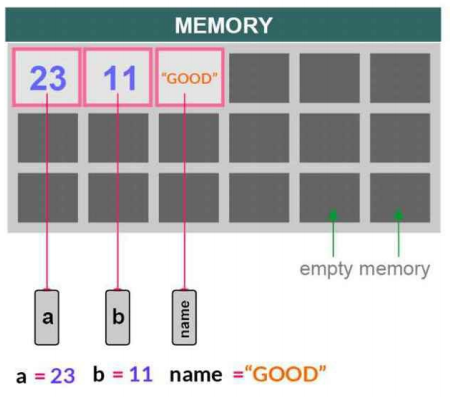
\includegraphics[width=.8\textwidth]{mutable_first.png}
			\end{figure}
		\end{frame}
		
		\begin{frame}
			\frametitle{Mutability - Example}
			\begin{figure}[h]
				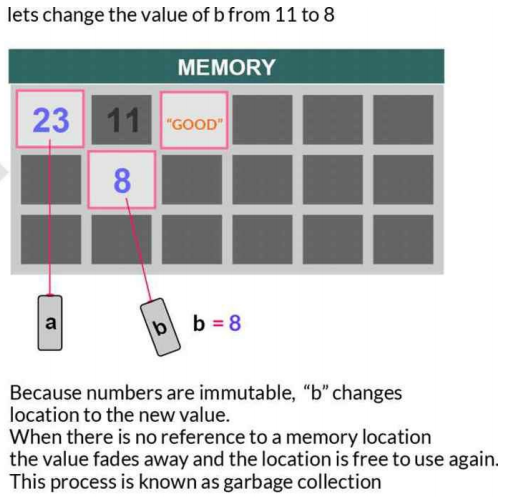
\includegraphics[width=.8\textwidth]{mutable_second.png}
			\end{figure}
		\end{frame}
		
		\begin{frame}
			\frametitle{Lecture 01 - Boolean and Numeric Types}
			\begin{itemize}
				\vfill\item  The concept of mutability isn't very important to us right now because of how transparent it is when using boolean and numeric type variables
				\vfill\item  Mutability will become more important to us when we start dealing with more complex types (strings, tuples, and lists)
				\vfill\item  Lets now play around with some more code to see how these boolean and numeric type variables work
					\begin{itemize}
						\item  Open up Lecture 01 - Boolean and Numeric Types.ipynb using jupyter notebooks
					\end{itemize}
			\end{itemize}
		\end{frame}
		
	\subsection{Basic Function}
	
		\begin{frame}
			\frametitle{Lecture 02 - Basic Functions}
			\begin{itemize}
				\vfill\item  At this point we can produce code to create a specif output, but if we want to repeat the same functionality with different input we would need to completely reproduce the code to do that
				\vfill\item  To speed along the process we can create what are called functions
				\vfill\item  Functions are blocks of code that can be reused by calling the function name and providing it some input
			\end{itemize}
		\end{frame}
	
		\begin{frame}
			\frametitle{Lecture 02 - Basic Functions}
			\begin{itemize}
				\vfill\item  We use the keyword \texttt{def} to create a function
				\vfill\item  \texttt{def}  is then followed by the new functions name
				\vfill\item  After the function name comes an open and close parenthesis (which can contain optional input variables) and a `:'
				\vfill\item  To get information back out of a function we use the keyword \texttt{return}
				\vfill\item  Lets walk through how to create some basic functions
				\vfill\item  Open up Lecture 02 - Basic Functions.ipynb using jupyter notebooks
			\end{itemize}
		\end{frame}
		
	\subsection{Control Flow}
	
		\begin{frame}
			\frametitle{Lecture 03 - Control Flow}
			\begin{itemize}
				\vfill\item  We now have convenient methods for reproducing code, however, are programs are currently static (meaning they aren't changing)
				\vfill\item  We need a way to change what a program does while it is executing
				\vfill\item  To do this we use what is called an if statements
				\vfill\item  In Python if statements must have an if statement (which evaluates to True or False)
				\vfill\item  If statements then also have optional pieces of elif and else
				\vfill\item  Lets look at how we can use if statements to change what our code does on the fly
				\vfill\item  Ope up Lecture 03 - Control Flow.ipynb using jupyter notebooks
			\end{itemize}
		\end{frame}
		
	\subsection{Sequences, Sets, and Mappings}
	
		\begin{frame}
			\frametitle{Lecture 04 - Sequences, Sets, and Mappings}
			\begin{itemize}
				\vfill\item  Sequences
					\begin{itemize}
						\item  Strings (Immutable)
							\begin{itemize}
								\item  A sequence of characters
							\end{itemize}
						\item  Tuples (Immutable)
							\begin{itemize}
								\item  A collection of mixed data types
							\end{itemize}
						\item  Lists (Mutable)
							\begin{itemize}
								\item A collection of mixed data types
								\item  Probably your most commonly used data structure
							\end{itemize}
					\end{itemize}
				\vfill\item  Sets
					\begin{itemize}
						\item  Sets (Mutable)
							\begin{itemize}
								\item  Unordered collection of data with no duplicates
							\end{itemize}
						\item  Frozen Sets (Immutable)
							\begin{itemize}
								\item  Unordered collection of data with no duplicates
							\end{itemize}
					\end{itemize}
				\vfill\item  Mappings
					\begin{itemize}
						\item  Dictionaries (Mutable)
							\begin{itemize}
								\item  A collection of key-value pairs
							\end{itemize}
					\end{itemize}
			\end{itemize}
		\end{frame}
		
	\subsection{Data I//O}
	
		\begin{frame}
			\frametitle{Lecture 05 - Data IO}
			\begin{itemize}
				\vfill\item  For other data analysis tools there are only a limited number of ways to open external data sources
				\vfill\item  Since Python is strongly focused on the use of external modules, there are a whole slew of methods for importing data
				\vfill\item  Depending on your particular application, you may want to use different import functions
				\vfill\item  In this quick class we will only focus on a few of some of the more widely used methods
			\end{itemize}
		\end{frame}
		
	\subsection{Loops}
	
		\begin{frame}
			\frametitle{Lecture 06 - Loops}
			\begin{itemize}
				\vfill\item  Python has two different types of loops that you can take advantage of
				\vfill\item  For loops
					\begin{itemize}
						\item  Iterates through a collection or iterable object
						\item  This will commonly be a list
					\end{itemize}
				\vfill\item  While loops
					\begin{itemize}
						\item  Loops while a conditions continues to be true
						\item  Stops when the condition becomes false
					\end{itemize}
			\end{itemize}
		\end{frame}
		
	\subsection{Advanced Functions}
	
		\begin{frame}
			\frametitle{Lecture 07 - Advanced Functions}
			\begin{itemize}
				\vfill\item  We have already created some rudimentary functions
				\vfill\item  Lets take some of the more advanced concepts we have learned and combine them with functions to make more complex and useful pieces of code
			\end{itemize}
		\end{frame}
		
	\subsection{Plotting}
	
		\begin{frame}
			\frametitle{Lecture 08 - Plotting}
			\begin{itemize}
				\vfill\item  One of the first things you want to do when you get a new data set is explore it
				\vfill\item  One of the best ways to do that is to plot the data in a variety of ways to see what types of patterns exist in it
				\vfill\item  The most common plotting tool in Python is matplotlib
				\vfill\item  Lets look as some simple matplotlib examples to see what we can create
				\vfill\item  Lets also look at another data exploration tool Seaborn to see what else is out there
			\end{itemize}
		\end{frame}
		
	\subsection{Regression}
	
		\begin{frame}
			\frametitle{Lecture 09 - Regression}
			\begin{itemize}
				\vfill\item  Regression is one of the most commonly used prediction methods in data science
				\vfill\item  There are a large number of programs dedicated to performing only regression analysis
				\vfill\item  There are also a large number of Python packages dedicated to regression analysis
				\vfill\item  One of the easiest to use, and which uses the same format as R, is Statsmodels
				\vfill\item  Lets look at a few examples of how we can use statsmodels for regression
			\end{itemize}
		\end{frame}
		
	\subsection{Data Science}
	
		\begin{frame}
			\frametitle{Lecture 10 - Data Science}
			\begin{itemize}
				\vfill\item  We have now covered:
					\begin{itemize}
						\item  Basic Python data structures
						\item  Functions
						\item  Program control flow
						\item  Data I/O
						\item  Loops
						\item  Plotting
						\item  Regression
					\end{itemize}
				\vfill\item  Lets now try to combine some of these tools, and some data science, into some useful analytics applications
			\end{itemize}
		\end{frame}
		
\section{Conclusion}

	\begin{frame}
		\frametitle{Conclusion}
		\begin{itemize}
			\item  I hope I have helped you to learn some very basic Python programming today
			\item  We went through a lot of material very quickly, so don't feel bad if you didn't catch everything
			\item  If you want to learn to program I would recommend Python as a first programming language
			\item  Python is also a power tool for data analytics and general purpose programming
			\item  If you want to learn more about Python there are a large number of useful resources as books, online tutorials, and online courses
			\item  If you have any pressing questions, you can reach out to me at:
				\begin{itemize}
					\item  \href{mailto:andrewarmstrong004@gmail.com}{andrewarmstrong004@gmail.com}
				\end{itemize}
		\end{itemize}
	\end{frame}
		

\end{document}